\chapter{晶体的范性变形}
    当金属和合金受力时首先产生弹性变形,以后再开始进入塑性变形(或称范性变形)。塑性变形继续进行直到材料发生
    断裂之前的过程称为流变过程。在流变过程中材料受力与变形的相互对应关系对了解材料的内部特性非常重要,因此
    测量并分析材料的应力应变曲线也是关键的一步。一般材料的应力应变曲线的测定要遵循国标,
    其中关键的控制因素就是应变速率要一定。

    如果定义试样的原始横截面积$A_0$,瞬时横截面积为$A_i$,原始长度为$l_i$,
    断口横截面积为$A_f$,试样所受载荷为$P$,可以得到工程应力应变和真实应力应变。

    假设试样在拉伸过程中体积不发生改变,此时计算出的应力和应变为工程应力\index{工程应力}$\sigma_e$和工程应变\index{工程应变}$\varepsilon_e$有如下定义:
    \begin{align}
        \sigma_{e}&=\frac{P}{A_0},\\
        \varepsilon_{e}&=\frac{\Delta l}{l_0},
    \end{align}
    但是在拉伸过程中,试样会出现颈缩现象,这与假设不符,因此又引入了工程应力\index{真实应力}$\sigma_t$和工程应变\index{真实应变}$\varepsilon_t$:
    \begin{align}
        \sigma_{t}&=\frac{P}{A_i},\\
        \varepsilon_{t}&=\ln\left( \frac{l_0}{l_i} \right).
    \end{align}

    根据两种不同的定义,将实验中得到的拉应力和试样的形变量作出对应的曲线也有两种,
    分别为工程应力应变曲线\index{工程应力应变曲线}和真实应力应变曲线\index{真实应力应变曲线}。

    对于工程应力应变曲线,在开始阶段呈线性变化,金属内部仍为弹性变形。
    。应力达到屈服应力时出现锯齿状平台,而后发现应力虽应变增加而增加阶段,是为加工硬化阶段。
    然而当应力越过最高点后会有一个下降段直到断裂。部分材料在拉伸过程中的屈服平台和
    屈服点都不明显,人为定义永久塑性形变为0.2\%时的应力为屈服点,用$R_{p0.2}$表示。
    工程应力应变曲线虽然不能反映实际的应力应变,但是操作比较简单,因此被广泛使用。

    对于真实应力应变曲线\index{真实应力应变曲线},也分为两段,首先也是线性变化,而后逐渐偏离
    直线过渡到向上弯曲,即弹性变形。在真实应力应变曲线上,没有明显屈服点,但是有两个应力需要注意,
    一是弹性极限$\sigma_{\mathrm{p}}$,即应力小于$\sigma_{\mathrm{p}}$时,只有弹性形变,另一个
    也是人为规定的应力,这里不作介绍。从应力应变曲线上求出曲线包围的面积,也就是变形所作的功,
    这一个值定义为材料的韧性,也是断裂过程所吸收的能量。

    研究发现,试样开始屈服到发生颈缩,阵营里应变满足经验关系
    \begin{equation}
        \sigma=K\varepsilon^n,
    \end{equation}
    $n$为加工硬化指数\index{加工硬化指数},$K$为强度系数,对上式取对数得到
    \begin{equation}
        \ln\sigma=\ln K+n\ln\varepsilon, 
    \end{equation}
    $n$在数值上等于试样的均匀变形量。不同的材料如果根据直线斜率$n$分为
    \begin{itemize}
        \item 理想弹性体,$n=1$,真应力应变曲线的斜率为1;
        \item 理想塑性体,$n=0$,真应力应变曲线为水平直线;
        \item 一般材料,$0<n<1$,曲线斜率在0到1之间。
    \end{itemize}
    \section{单晶体的滑移变形}
        前面已经提到,位错的滑移可以引发材料发生塑性变形,因此材料的塑性变形方
        式包括位错的滑移,孪生;高温状态下还会有晶界滑动方式。
        \subsection{滑移晶体学特征}
            位错滑出晶体后,会在晶体表面造成台阶,早期的研究发现,相同点阵结构的材
            料其相互错动的晶面(也就是位错的滑移面),错动方向称为滑移方向,总是有确定的
            指数,定义一个滑移面和一个滑移方向构成1 个滑移系。

            人们发现滑移面,即能够发生滑移的晶面,往往是原子密排面,这与位错滑移的
            点阵阻力较小有关,在滑移面上按一定晶向进行的滑移方向,是原子的密排方向。
            \autoref{常见的几种点阵类型的滑移系统}总结处常见的几种点阵类型的滑移系统。
            \begin{table}[ht]
            \centering
            \caption{常见的几种点阵类型的滑移系统。}
            \label{常见的几种点阵类型的滑移系统}
            \begin{tabular}{ccccc}
            \toprule
            &滑移面&滑移方向&滑移系个数&条件\\
            \midrule
            FCC&$\left\{ 111\right\}$& $\langle 111 \rangle$ &12& \\
            \multirow{3}*{BCC}&$\left\{ 110\right\}$&\multirow{3}*{$\langle 111 \rangle$}&12&\\
            &$\left\{ 112\right\}$&&12&\\
            &$\left\{ 123\right\}$&&24&\\
            \multirow{2}*{HCP}&$\left\{ 0001\right\}$&$\langle 11\bar{2}0 \rangle$&3&$c/a>1.633$\\
            &$\left\{ 10\bar{1}0\right\}$&$\langle 11\bar{2}0 \rangle$&3&$c/a<1.633$\\
            \bottomrule
            \end{tabular}
            \end{table}
        \subsection{影响滑移系统的因素}
            研究发现,滑移系统不仅与晶体的点阵类型有关,而且还受到其它因素的影响:
            \begin{enumerate}
                \item 温度:当温度升高时,滑移系也增加;
                \item 应变速率:应变速率增大相当于温度降低,滑移系有可能减少;
                \item 合金化元素对不同晶体结构影响不同:
                \begin{enumerate}
                    \item 面心立方加入合金化元素一般对滑移系不产生影响;
                    \item 体心立方加入合金化元素后,对48个滑移系产生选择性;
                    \item 合金化元素对六方结构的影响取决于$c/a$的比值变化。 
                \end{enumerate}
            \end{enumerate}
        \subsection{滑移方式与滑移带}
            实验表明,材料发生范性形变之后,用光学显傲镜观察变形晶体的表面时常常看到一些线状痕迹,如
            如\autoref{单相黄铜中的滑移带}所示。
            这些痕迹是滑移面和晶体外表面的交钱,称为滑移线。如果进一步放大观察,
            可以发现滑移线有精细结构,用电子显微镜观察变形晶体的表面时发现,原来用光学显微镜观察到的
            “滑移线”实际上是由彼此靠近的一组滑移线构成的,称为滑移带。

            在形变过程中,滑移带中,滑移线间没有发生滑动的中间区域叫做滑移层,它们的宽度一般在几十个纳米之间。
            \begin{figure}[ht]
                \centering
                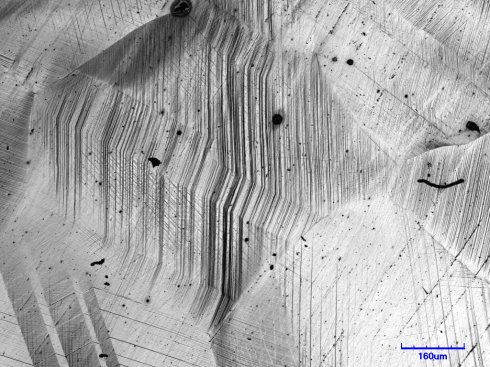
\includegraphics[width=0.5\textwidth]{fig/slip_band_twin_crystal.png}
                \caption{单相黄铜中的滑移带,滑移带在孪晶的位置会发生弯折。图片来源于\href{http://blog.sina.cn/dpool/blog/s/blog_674374ae0101dz8p.html}{quantimet720金相技术}的博客}
                \label{单相黄铜中的滑移带}
            \end{figure}
            
            根据材料中动作的滑移系的状况可以定义:
            \begin{itemize}
                \item 单滑移:只有一个滑移系动作;
                \item 双滑移:两个滑移系同时开动;
                \item 多滑移:多个滑移系同时开动;
                \item 铅笔型滑移:滑移线由具有共同滑移方向的若干滑移面的滑移所组成,(bcc晶体中,多个滑移面向单方向滑移)也称为交叉滑移\footnote{注意不是交滑移,交滑移是指螺位错变换滑移面。}。
            \end{itemize}
    \section{单晶体屈服与晶体的转动及碎化}
        \subsection{临界分切应力定律}
            人们发现,要使单晶体发生滑移,在滑移系上作用的切应力必须达到一个临界值,
            与在该晶面上作用的正应力无关。这个切应力成为临界分切应力。

            当拉伸轴与单晶体的位相关系已知,可以计算作用在滑移系上的分切应力。 
            
            临界分切应力大小与杂质的关系很大也与温度有关。温度升高,临界分切应力下降,
            其下降速率随温度升高而降低,不同滑移系的临界分切应力随温度的升高而趋同。
        \subsection{临界切应力的位错理论}
            晶体收到外应力作用,取向因子最大的滑移系位错开始滑移,其他位错或晶体缺陷要对它的运动产生
            阻碍或交互作用,主要考虑以下几种
            \begin{enumerate}
                \item[1] 位错增殖;
                \item[2] 点阵阻力;
                \item[3] 与其他位错的交互作用:
                \begin{enumerate}
                    \item[1] 弹性应力场的交互作用。为了简便起见,设有二个位错排列在垂直的方向,相距为l。位错要从B、C中间穿过去,就要克服B、C的长程弹性作用力。假设平行于可动位错的那些位错均匀分布,这些位错之间的间距用$l_1$表示,可以推导得出:位错克服的应力为$\tau=\alpha\mu b\sqrt{\rho}$。
                    \item[2] 位错塞积;塞积导致应力集中\footnote{如果塞积群与所求位错之间距离较远,可以视塞积群为一个扩大$N$倍的柏式矢量,其中$N$为塞积群位错数量。}。位错受到的阻力为$\tau_0^2=\alpha\frac{\mu b}{l_2}$
                    \item[3] 位错绕过位错林;与增殖过程相似,在林位错周围形成位错环,然后继续滑移,阻碍切应力为$\tau_0^3=\alpha\frac{\mu b}{l_2}$;
                    \item[4] 以上的三个$\alpha$并非同一常数,仅仅为方便使用同一符号,而且以上的阻力与位错的温度没有关系,
                    \item[5] 切过林位错产生交割,这一部分是短程相互作用,与热激活有关,这是温度升高,屈服强度降低的原因。外力为$\tau$,长程应力为$\tau_0$,外力完成完全切割做功为$W=(\tau-\tau_0)bld$,产生割阶的能量为$\Delta H_0$,热激活提供的能量为$\Delta H=\Delta H_0-(\tau-\tau_0)bld$,当温度高于一定值,形成割阶的能量完全由热激活提供,不需要外力。
                \end{enumerate} 
            \end{enumerate}
            提高屈服强度也就是提高位错运动的长程和短程阻力,主要有以下途径:
            \begin{itemize}
                \item[1] 位错密度上升,比如通过拉拔进行加工硬化,桥梁钢在处理后屈服强度可提升50\%;
                \item[2] 障碍物尺寸增加;
                \item[3] 障碍物间距缩小,也就是增加障碍物密度,比如弥散强化;
                \item[4] 障碍物的稳定性增加。
            \end{itemize}
            影响临界分切应力$\tau_0$的因素
            \begin{itemize}
                \item[1] 高温段不发生变化,温度降低,应力上升,对韧性产生影响;
                \item[2] 合金元素的存在,一般会使临界切应力$\tau_0$增加;
                \item[3] 应变使位错密度增加,进而也会使切应力增加;
            \end{itemize}
        \subsection{拉伸过程中晶体的转动和碎化}
            滑移面与拉伸轴不平行,切变方向沿滑移方向,无法沿拉伸轴方向,因此,试样两端会产生位移。在拉伸实验中,两端被限制,晶面会受到转动力矩的作用,从而发生转动。

            在不能整体发生倾转的时候,表面出现$S$状的滑移线,同号的位错堆积起来,然后产生晶体弯曲,变形过程中晶体的碎化,在取向差小于\ang{15}时\footnote{小角晶界处。},将会出现亚晶。
            产生畸变后,在衍射斑上会出现星芒。
        \subsection{孪生}
            孪生是晶体塑性变形的另一种方式,比如,体心立方的金属的六个偏位错滑移产生孪晶,当晶体的一部分相对另一部分呈镜面对称时,两者互为孪晶。
            
            其与滑移的差异
            \begin{itemize}
                \item[1] 原子到孪生面的移动距离不是常数;
                \item[2] 抛光之后仍然可见;而滑移是表面现象,内部不产生畸变,而孪生不会因为抛光改变晶体排列,仍然可见;
                \item[3] 形状通常为薄透镜状;
                \item[4] 发生速度可以很快;
                \item[5] 一般是滑移受阻时产生的。
            \end{itemize}
        \subsection{总结}
            单晶体塑性变形的三个过程:1.切变,2.转动,3.碎化。
    \section{多晶体范性变形的特点及晶界的作用}
        \subsection{多晶体塑性变形的特点}
            一般情况下,多晶材料屈服应力大于单晶材料,因为晶界会产生强化效应。
            在若干晶系中,选择$\omega$最大的取向最先发生开动,晶粒中发生多滑移,使其发生变形的方向一致。二这需要至少五个滑移系同时运动。
            这也是多晶变形的特点之一:多滑移。

            在晶界附近,为位错滑移受到阻碍,发生位错塞积。

            在变形过程中,会出现择优取向,也就是织构。
        \subsection{多晶体的屈服应力}
            假设在A 晶粒中的某个滑移系处于有利的取向,其取向因子最大,也最先开始滑
            移,滑移后位错遇到晶界,位错塞积,之后在B晶粒的晶界处产生应力集中,当应力集中过大时,
            B中的滑移系达到了临界应力,也会发生滑移,变形也就从$A$传递到了$B$。这是变形的传递过程。

            假设A晶粒中的变形可以表示为
            \begin{equation}
                \gamma=\frac{nb}{L},
            \end{equation}
            其中$L$为A晶粒的滑移方向的长度,
            此时B晶粒没有发生位错滑移,仍然处于弹性变形阶段,所以B中的切应力为
            \begin{equation}
                \gamma^{\prime}=\frac{\tau}{\mu},
            \end{equation}
            两个晶粒的应变应当相同,也就是$\gamma=\gamma^{\prime}$,也就是
            \begin{equation}
                \frac{nb}{L}=\frac{\tau}{\mu},
            \end{equation}
            所以晶界处的位错数为
            \begin{equation}
                n=\frac{\tau L}{\mu b},
            \end{equation}
            位错开始开动时,需要临界分切应力等于该处的集中的应力,因此有
            \begin{equation}
                \tau_c=\frac{n\tau}{\alpha}=\frac{\tau^2L}{\alpha\mu b},
            \end{equation}
            此时外加应力为
            \begin{equation}
                \tau=\sqrt{\frac{\alpha\mu b\tau_c}{L}}=k\cdot L^{-\frac{1}{2}},
            \end{equation}
            屈服应力为
            \begin{equation}
                \tau=\tau_0+k\cdot L^{-\frac{1}{2}},
            \end{equation}
            其中$L$为晶粒尺寸,$\tau_0$为晶格摩擦阻力,$k$为常数,$L$为平均晶粒尺寸。
